\section{Apresentação da Proposta}
\label{sec:apresentacao-proposta}

Conforme apresentado na Seção \ref{sec:data-preproces}, a etapa de pré\hyp{}processamento é de grande importância na descoberta de conhecimento em bases de dados. Em seu decorrer é possível analisar a estrutura destes dados e aplicar as correções necessárias, para que algoritmos de mineração possam extrair padrões de conhecimento considerados úteis à partir das coleções. A execução desta etapa não é um processo simples, deve ser considerada a variedade de erros que possam existir nas amostras trabalhadas, pois diversos métodos podem ser aplicados a fim de solucionar ou suavizar tipos individuais de erros.

\begin{figure}[H]
    \centering
    \caption{Proposta metodológica.}
    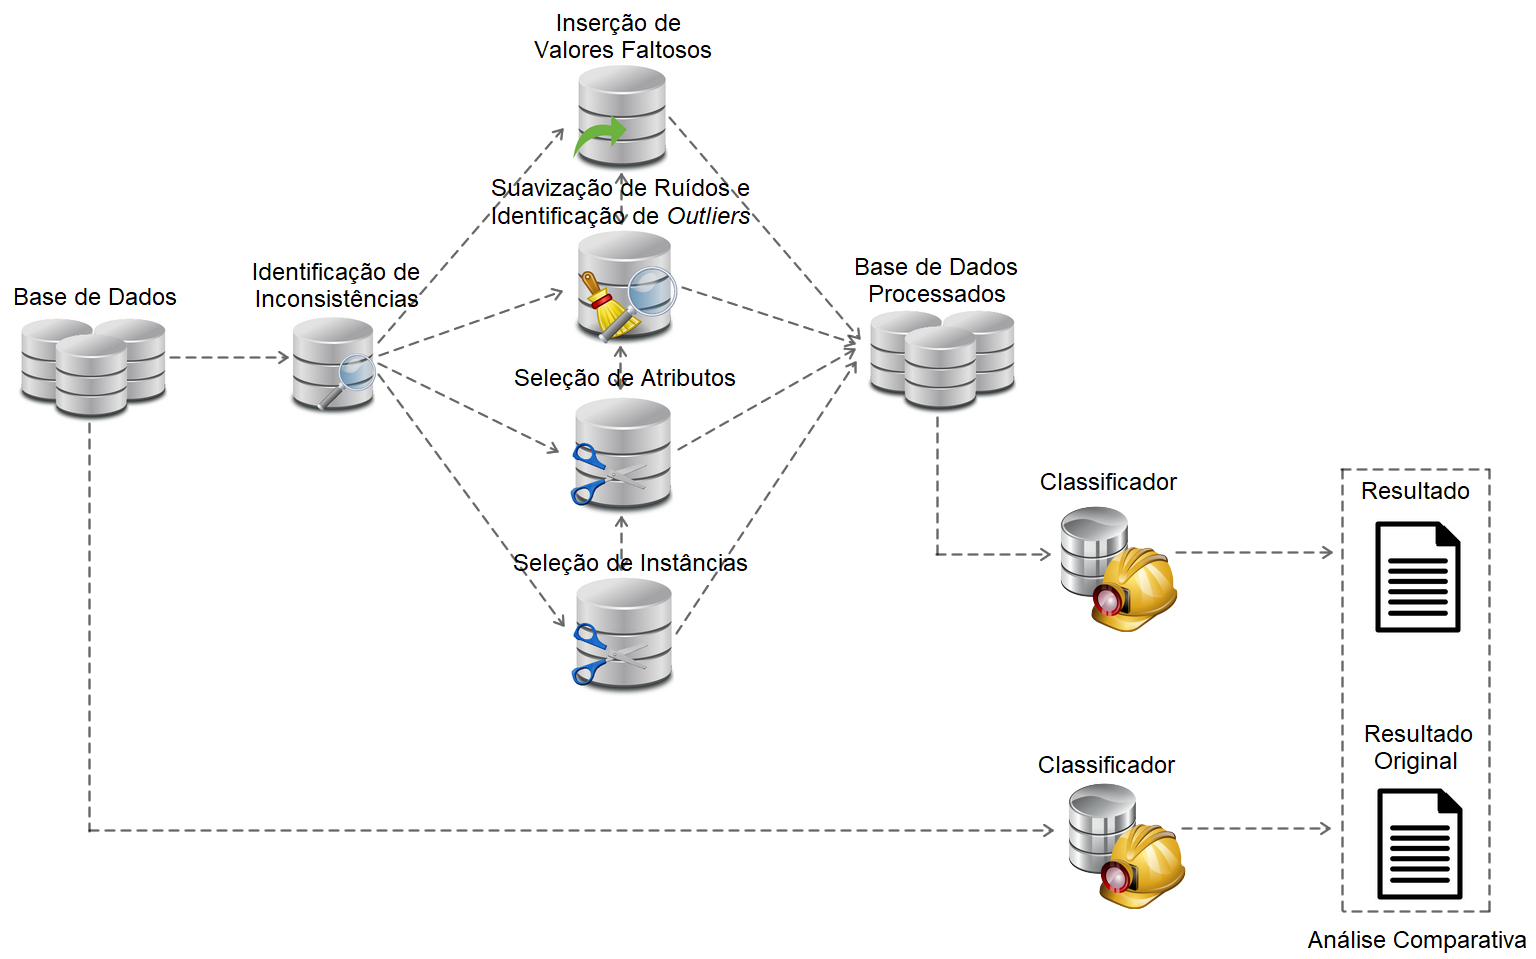
\includegraphics[width=\linewidth]{figuras/modelo-proposta.png}
    \source{Próprio autor (2017).}
    \label{fig:proposta-metodologica}
\end{figure}

Este trabalho busca identificar possíveis erros e aplicar técnicas de pré\hyp{}processamento à fim de corrigir as inconsistências encontradas em dados à serem coletados através da aplicação de jogos sérios à crianças de faixa etária entre 7 e 12 anos. O objetivo final é obter um conjunto de dados que proporcione maior acurácia e desempenho em algoritmos classificação, proporcionando uma base de dados adequados aos comitês de classificadores citados na Seção \ref{sec:delimitacao-estudo}. A Figura \ref{fig:proposta-metodologica} ilustra o processo envolvido neste trabalho, desde a coleta da base até a validação dos resultados obtidos pelo classificador.